% !TEX root = SFV-15014_HuV.tex
\section{Einf\"uhrung}
\begin{frame} % Cover slide
\titlepage
\end{frame}

\frame{\sectionpage}
\offslide{Mindmap Vorlesungsinhalte}

\frame[allowframebreaks]{
\frametitle{Inhalt der Vorlesung}
\tableofcontents
}



\frame{\frametitle{Themenplan}
\framesubtitle{Nutzen Sie die als E-Book verf\"ugbaren Literaturempfehlungen zu diesem Modul! Vor der Vorlesung! Das Buch \citep{schindler} ist nur als Printversion verf\"ugbar.}
\begin{center}
\tiny
%\hspace{2cm}
\begin{tabular}{|c|l|l|}
\hline
KW & Thema & Literaturempfehlung \\ \hline
13 & Pr\"aliminarien & \\ \hline
14 & Marktsegmentierung und -grundlagen & \citep{unife12}  \\ %\hline
 & Marktbarrieren und -risiken &  \\ \hline
15 & Projektablauf, -kriterien, -organisation & \citep{felkai} 1 - 2.3 \\ \hline
16 &  Projektdokumentation & \citep{felkai} 2.4  \\ 
 & Vertragspr\"ufung & \citep{kanitzky} I.1, I.2, (I.3)  \\ \hline
17 & Requirements Engineering  & \citep{SEGuide} 3.1, 3.5 - 3.7 \\ %\hline
 & Aufwands- und Kostensch\"atzung & \citep{capone} 3.4 - 3.6 \\  \hline
%\color{gray!70} 20 & \color{gray!70} Exkursion (tbc)  &  \\ \hline
18 & Projektplanung &   \\ \hline 
19 & Rohbau & \citep{schindler} 6.1   \\  
& Grundlagen Lean Manufacturing & ? \\ \hline
& Klassifizierung nach EN15085 & (EN 15085-3)  \\
20 & Schwei{\ss}en an Schienenfahrzeugen & (EN 15085-4)   \\ 
& Aluminium und Stahl & (EN 15085-5)  \\ \hline
21 &  Schwei{\ss}en an Schienenfahrzeugen &  \\ 
& Festigkeitsberechnung & (DVS 1612)  \\ \hline
22 &  Schraubenverbindungen & (DIN 25201-1, 2, 4) \\ \hline
%\color{gray!70} 23 & \color{gray!70} Exkursion (tbc) & \\ \hline
23 & Materialien und Korrosionsschutz & \citep{schindler} 6.2  \\ 
& DB G\"utepr\"ufung &  \\\hline
24 &  Innenausbau & \citep{schindler} 6.3  \\ 
& Brandschutz &  \\ \hline
25 &  Fahrwerk und Rads\"atze & \citep{schindler} 6.4, 6.5 \\ \hline
26 & Inbetriebsetzung und Abnahme & \citep{schindler} 6.6  \\ \hline
\end{tabular}
\end{center}
}

\frame{\frametitle{Seminararbeiten}
\framesubtitle{Seminararbeiten sind eigenst\"andige wissenschaftliche Arbeiten.}
\begin{itemize}
\item Gewichtung: 30\% der Modulnote durch Seminararbeit
\item Anforderungen:
\begin{itemize}
		\item Erstellung von Projektdokumenten im Team
		\item Pr\"asentation
		\item Abgabe als Team
\end{itemize}
\end{itemize}
}


\frame{\frametitle{Praktikum}
\framesubtitle{Das Praktikumsvolumen wird teilweise in Form von Exkursionen, teilweise in Form von praxisnahen Arbeiten geleistet.}
\begin{itemize}
\item Termine folgen
\item Dokumentation des Praktikums durch technischen Bericht, Gewichtung Bericht: 20\% der Modulnote
\item 
\end{itemize}
}

\frame{\frametitle{Das Projekt - Team 1 - Betreiber}
\framesubtitle{Beschaffung einer vierachsigen Elektrolokomotive (im Ma{\ss}stab 1:32) f\"ur Messungen der L\"angsdynamik.}
\begin{columns}[t] 
     \begin{column}[T]{6cm} 
     \textbf{Aufgaben:}
     	\begin{enumerate}
     		\item Anforderungserhebung
		\item Erstellung Lastenheft Gesamtfahrzeug
		\item Erstellung Abnahme-Spezifikation
     	\end{enumerate}
     \end{column}
     	\begin{column}[T]{6cm} 
         	\begin{center}
            		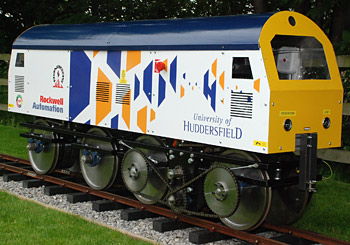
\includegraphics[width=0.8\textwidth]{Lok}
        		\end{center}
     \end{column}
 \end{columns}
}

\frame{\frametitle{Das Projekt - Team 2 - Fahrzeugbauer / Vertrieb}
\framesubtitle{Umsetzungsplanung f\"ur eine vierachsige Elektrolokomotive (im Ma{\ss}stab 1:32) f\"ur Messungen der L\"angsdynamik.}
\begin{columns}[t] 
     \begin{column}[T]{6cm} 
     \textbf{Aufgaben:}
     	\begin{enumerate}
		\item Clause-by-Clause-Kommentierung Lastenheft Gesamtfahrzeug
		\item Erstellung technisches Angebot
     	\end{enumerate}
     \end{column}
     	\begin{column}[T]{6cm} 
         	\begin{center}
            		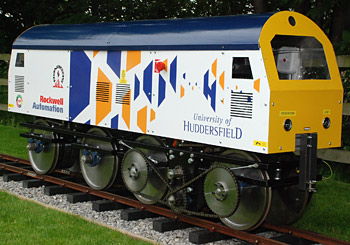
\includegraphics[width=0.8\textwidth]{Lok}
        		\end{center}
     \end{column}
 \end{columns}
}

\frame{\frametitle{Das Projekt - Team 3 - Fahrzeugbauer / Technik}
\framesubtitle{Umsetzungsplanung f\"ur eine vierachsige Elektrolokomotive (im Ma{\ss}stab 1:32) f\"ur Messungen der L\"angsdynamik.}
\begin{columns}[t] 
     \begin{column}[T]{6cm} 
     \textbf{Aufgaben:}
     	\begin{enumerate}
		\item Erstellung Pflichtenheft Gesamtfahrzeug
		\item Erstellung Lastenheft Drehgestell
     	\end{enumerate}
     \end{column}
     	\begin{column}[T]{6cm} 
         	\begin{center}
            		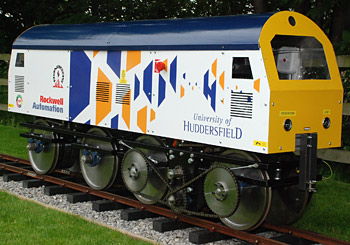
\includegraphics[width=0.8\textwidth]{Lok}
        		\end{center}
     \end{column}
 \end{columns}
}

\frame{\frametitle{Das Projekt - Team 4 - Drehgestell / Vertrieb}
\framesubtitle{Umsetzungsplanung f\"ur eine vierachsige Elektrolokomotive (im Ma{\ss}stab 1:32) f\"ur Messungen der L\"angsdynamik.}
\begin{columns}[t] 
     \begin{column}[T]{6cm} 
     \textbf{Aufgaben:}
     	\begin{enumerate}
		\item Clause-by-Clause-Kommentierung Lastenheft Drehgestell
		\item Erstellung technisches Angebot Drehgestell
     	\end{enumerate}
     \end{column}
     	\begin{column}[T]{6cm} 
         	\begin{center}
	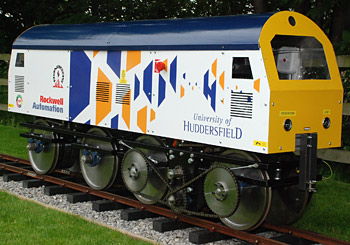
\includegraphics[width=0.8\textwidth]{Lok}
        		\end{center}
     \end{column}
 \end{columns}
}
